\subsection{Vývojové prostredie a platforma}

\subsubsection{Operačný systém Android}
Táto práca je zameraná na vývoj mobilnej aplikácie pre operačný systém \textbf{Android}. Dôvodom zvolenia tejto platformy je jej dominantné postavenie na trhu mobilných zariadení, kde podľa aktuálnych štatistík zaujíma viac ako 70 \% podiel. Android ponúka široké možnosti prispôsobenia a hlbokej integrácie s hardvérovými službami (ako sú lokalizačné služby), čo je kľúčové pre praktickú časť tejto práce.
\\ (Zdroj: \url{https://gs.statcounter.com/android-version-market-share})

\subsubsection{Distribúcia a ekosystém platforiem}
Voľba operačného systému ovplyvňuje nielen technologický zásobník, ale aj stratégiu uvedenia na trh. Platforma Android je často preferovaná pre nasadenie minimálneho životaschopného produktu (\textit{MVP}) kvôli flexibilnejším pravidlám v obchode Google Play v porovnaní s uzavretým ekosystémom iOS.

Hoci existujú multiplatformové riešenia, pre účely tejto práce bol zvolený natívny prístup z dôvodu maximálnej optimalizácie výkonu a prístupu k systémovým API. Porovnanie prístupov na základe analýzy \cite{pullur_medium_2025} uvádza Tabuľka \ref{tab:final_comparison}.

\begin{table}[h!]
\centering
\caption{Súhrnné porovnanie natívneho a multiplatformového vývoja}
\label{tab:final_comparison}
\resizebox{\textwidth}{!}{%
\begin{tabular}{|l|c|c|c|c|}
\hline
\textbf{Metrika} & \textbf{Native (Kotlin)} & \textbf{Flutter} & \textbf{React Native} & \textbf{KMM} \\ \hline
Veľkosť aplikácie & \textbf{Najmenšia} & Väčšia & Väčšia & Stredná \\ \hline
Rýchlosť štartu & \textbf{Najrýchlejšia} & Stredná & Pomalšia & Rýchla \\ \hline
Animácie & \textbf{Plynulé} & Plynulé & Riziko lagov & -- \\ \hline
Zdieľanie kódu & Žiadne & 95 \% + & 90 \% + & Logika \\ \hline
Spotreba batérie & \textbf{Nízka} & Stredná & Vysoká & Nízka \\ \hline
\end{tabular}%
}
\end{table}

\subsection{Programovací jazyk Kotlin}
Kotlin je moderný, staticky typovaný jazyk, ktorý je od roku 2019 preferovanou voľbou spoločnosti Google pre vývoj aplikácií na platformu Android. Medzi jeho kľúčové prínosy pre túto prácu patria:

\begin{itemize}
    \item \textbf{Null Safety:} Výrazne znižuje riziko pádov aplikácie (chyba \textit{NullPointerException}) vďaka striktnému rozlišovaniu nulovateľných typov už v čase kompilácie.
    \item \textbf{Coroutines:} Umožňujú efektívne vykonávanie asynchrónnych úloh (napr. sťahovanie dát o podujatiach z cloudu) bez blokovania hlavného vlákna a zamŕzania používateľského rozhrania.
    \item \textbf{Stručnosť:} Redukcia nadbytočného kódu (\textit{boilerplate}) umožňuje rýchlejšiu implementáciu biznis logiky odporúčacieho algoritmu.
\end{itemize}


% (Zdroj: \url{https://developer.android.com/kotlin})

\subsection{UI Toolkit: Jetpack Compose}
Na tvorbu používateľského rozhrania bol zvolený moderný deklaratívny toolkit \textbf{Jetpack Compose}. Na rozdiel od staršieho systému založeného na XML súboroch, Compose umožňuje definovať UI priamo v jazyku Kotlin.

\begin{itemize}
    \item \textbf{Deklaratívny prístup:} Programátor opisuje výsledný stav rozhrania, pričom framework sa automaticky stará o jeho prekreslenie pri zmene dát (napr. pri aktualizácii zoznamu podujatí).
    \item \textbf{Komponentový dizajn:} UI je vyskladané z malých, znovupoužiteľných funkcií (\textit{Composables}), čo uľahčuje údržbu a testovanie aplikácie.
\end{itemize}
% (Zdroj: \url{https://developer.android.com/compose})


\subsection{Vývojové nástroje}
Android Studio je oficiálne vývojové prostredie (IDE) bohaté na funkcie pre vývoj aplikácií pre Android, ktoré integruje nástroje na návrh, kódovanie, tvorbu a testovanie.
Ponúka natívnu podporu pre Kotlin, Java a C++, rozsiahlu rozšíriteľnosť pluginov a bezproblémovú emuláciu naprieč typmi zariadení.
Pravidelné aktualizácie zabezpečujú kompatibilitu s novými verziami systému Android, pokročilé ladenie a analýzu výkonu v jednotnom prostredí a preto je ideálnou voľbou pre tento projekt.
% (Zdroj: \url{https://developer.android.com/studio})
% https://www.ikkaro.net/sk/what-is-android-studio/

\subsection{Technická špecifikácia a použité knižnice}

V tejto časti si spravil kus dobrej roboty, ale ak ideme podľa tvojho plánu (najprv vymazať zbytočné, potom skracovať), máme tu jasných kandidátov na "vyhadzov".

1. Čo je v tejto časti úplne zbytočné (MAZAŤ):
Definícia Android SDK: Vety o tom, že SDK obsahuje knižnice a emulátory a slúži na transformáciu kódu do balíka, sú veta pre prvákov. V inžinierskej práci o mobilnom vývoji sa predpokladá, že čitateľ vie, čo je SDK.

Verdikt: Vymaž celú prvú podkapitolu \subsubsection{Android SDK a správa verzií}. Nechaj len tie odrážky s verziami.

Marketingové reči o Material Design 3: Vety typu „...podporuje osvedčené postupy“, „...zefektívnenie spolupráce medzi dizajnom a vývojom“ alebo „...rýchle budovanie estetických produktov“ sú čistý marketingový text z webu Googlu.

Verdikt: Tieto vety letia von. Sú to prázdne frázy, ktoré oponent vníma ako vatu.

Definícia "targetSdk": Vysvetľovanie rozdielu medzi minSdk a targetSdk (posledný odsek pod odrážkami) je v diplomovke nepotrebné.

Verdikt: Vymaž tento vysvetľujúci odsek.

2. Ako to bude vyzerať po vymazaní (len čisté fakty):
Tento text má teraz polovicu dĺžky, ale dvojnásobnú informačnú hodnotu:

Útržok kódu
\subsection{Technická špecifikácia a dizajn}

\subsubsection{Konfigurácia Android SDK}
V rámci projektu sú definované úrovne rozhraní API, ktoré určujú rozsah kompatibility a dostupné systémové funkcie:
\begin{itemize}
    \item \textbf{minSdk 26 (Android 8.0):} Zvolené ako optimálny kompromis pre podporu moderných API (notifikačné kanály, JobScheduler) pri zachovaní pokrytia nad 90 \% zariadení.
    \item \textbf{targetSdk 35 (Android 15):} Zabezpečuje súlad s najnovšími bezpečnostnými štandardmi a protokolmi ochrany súkromia vyžadovanými pre Google Play.
\end{itemize}

\subsubsection{Vizuálne rozhranie Material Design 3}
Používateľské rozhranie je postavené na štandarde \textbf{Material Design 3} s využitím knižnice \texttt{androidx.compose.material3}. Hlavné prínosy integrácie zahŕňajú:
\begin{itemize}
    \item \textbf{Komponenty:} Využitie systémových prvkov ako \texttt{ModalNavigationDrawer} pre navigáciu a \texttt{ElevatedCard} pre zobrazenie detailov podujatí.
    \item \textbf{Adaptivita:} Natívna podpora pre rôzne hustoty pixelov a orientácie displeja.
    \item \textbf{Dynamické témy:} Podpora pre \textit{Material You}, umožňujúca prispôsobenie farebnej palety aplikácie nastaveniam systému.
\end{itemize}

% Zdroj: https://m3.material.io/get-started
% Zdroj: https://developer.android.com/develop/ui/compose/designsystems/material3
%pregenerovane geminy ai po vete vies to nejak skratit


\subsection{Externé softvérové knižnice}
Pre rozšírenie základných funkcií systému Android a zabezpečenie plynulého používateľského zážitku boli do projektu integrované špecializované knižnice. Tieto nástroje riešia kritické úlohy od navigácie v deklaratívnom prostredí až po nízkoúrovňovú komunikáciu s hardvérom kamery.

\subsubsection{Navigation Compose (2.8.5)}
Knižnica \textbf{Navigation Compose} poskytuje infraštruktúru pre riadenie toku obrazoviek v aplikáciách postavených na Jetpack Compose. Umožňuje definovať navigačný graf priamo v kóde Kotlin, čím nahrádza staršie riešenia založené na XML súboroch a fragmentoch.
\begin{itemize}
    \item \textbf{NavHost:} Slúži ako vizuálny kontajner, ktorý dynamicky vymieňa jednotlivé kompozitné funkcie (\textit{composables}) na základe aktuálnej trasy.
    \item \textbf{NavController:} Centrálny objekt, ktorý spravuje zásobník obrazoviek (\textit{backstack}) a zabezpečuje správnu reakciu na systémové tlačidlo „Späť“.
    \item \textbf{Typová bezpečnosť:} Verzia 2.8.5 prináša natívnu podporu pre typovo bezpečnú navigáciu, čo eliminuje chyby pri prenose argumentov (napr. ID podujatia) medzi obrazovkami.
\end{itemize}
% Zdroj: https://developer.android.com/develop/ui/compose/navigation

\subsubsection{CameraX (1.3.4)}
\textbf{CameraX} je moderná knižnica zameraná na prácu s fotoaparátom, ktorá odstraňuje zložitosť spojenú so správou špecifík hardvéru od rôznych výrobcov. Je postavená na koncepte prípadov použitia (\textit{use-cases}), z ktorých boli v projekte implementované najmä:
\begin{itemize}
    \item \textbf{Preview:} Zabezpečuje plynulý živý náhľad obrazu z kamery priamo v používateľskom rozhraní.
    \item \textbf{Image Analysis:} Poskytuje prístup k obrazovým dátam v reálnom čase, čo je kľúčové pre \textbf{algoritmy na skenovanie a dekódovanie QR kódov} pri vstupe na podujatia.
    \item \textbf{Image Capture:} Umožňuje zachytávanie fotografií (napr. pre profilové fotky alebo dokumentáciu podujatia) s automatickou optimalizáciou expozície a zaostrenia.
\end{itemize}
% Zdroj: https://developer.android.com/media/camera/camerax

\subsubsection{Coil (2.7.0)}
Názov \textbf{Coil} predstavuje akronym pre \textit{Coroutine Image Loader}. Ide o efektívnu knižnicu na asynchrónne načítavanie obrázkov z cloudu (Firebase Storage), ktorá je plne optimalizovaná pre prostredie Kotlin Coroutines.
\begin{itemize}
    \item \textbf{Optimalizácia výkonu:} Knižnica automaticky vykonáva operácie ako cachovanie na disk a do pamäte RAM, zmenu mierky obrázkov (\textit{downsampling}) a inteligentné rušenie sieťových požiadaviek pri odscrollovaní prvku z obrazovky.
    \item \textbf{Integrácia s Compose:} Vďaka natívnej podpore pre Jetpack Compose umožňuje zobrazenie obrázkov s minimálnym množstvom riadiaceho kódu (\textit{boilerplate}), čím zvyšuje čitateľnosť projektu.
\end{itemize}
% Zdroj: https://coil-kt.github.io/coil/


\subsection{Architektúra projektu}
V projekte využívame architektúru \textbf{MVVM} (\textit{Model-View-ViewModel}) v kombinácii s \textbf{Repository pattern}. 
Model MVVM pozostáva z troch základných komponentov, z ktorých každý má jasne definovanú zodpovednosť:
\begin{itemize}
    \item \textbf{Model:} Reprezentuje dátovú vrstvu a biznis logiku. V našom prípade sem patrí komunikácia s Firebase a správa lokálnych dát.
    \item \textbf{View (Zobrazenie):} Používateľské rozhranie, ktoré pasívne zobrazuje dáta a odosiela akcie používateľa do ViewModelu.
    \item \textbf{ViewModel (Model zobrazenia):} Pôsobí ako prostredník, ktorý pripravuje dáta z modelu pre zobrazenie a udržiava stav aplikácie nezávisle od životného cyklu rozhrania.
\end{itemize}

\begin{figure}[h!]
    \centering
    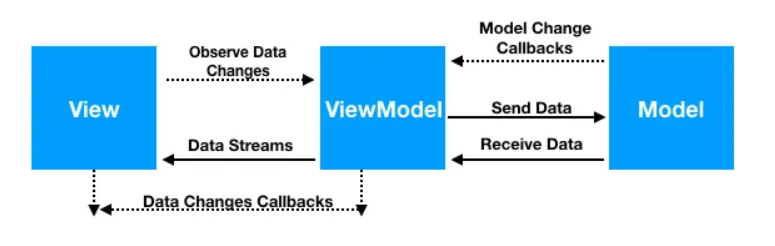
\includegraphics[width=0.8\textwidth]{img/MVVM}
    \caption{Diagram architektúry MVVM s Repository pattern v systéme Android}
    \label{fig:mvvm_architecture}
\end{figure}

Hlavným dôvodom voľby MVVM sú jeho prínosy pre stabilitu projektu, najmä \textbf{zvýšená testovateľnosť} (možnosť testovať logiku bez UI), \textbf{jednoduchšia údržba} vďaka oddeleniu zodpovedností a \textbf{odolnosť voči zmenám konfigurácie} (napr. otočenie displeja), kedy ViewModel chráni dáta pred stratou.
%https://medium.com/@zorbeytorunoglu/mvvm-in-android-059e9aae84c1
\subsubsection{Moderný prístup: MVVM v kombinácii s Jetpack Compose}
V súlade s princípmi čistého návrhu (\textit{Clean Architecture}) opísanými v \cite{sks_medium_2024}, je v projekte implementovaný vzor MVVM s dôrazom na \textbf{jednosmerný tok dát} (\textit{Unidirectional Data Flow - UDF}). Tradičný mechanizmus \textit{Data Bindingu} známy zo starších verzií Androidu je tu nahradený moderným reaktívnym prístupom:

\begin{itemize}
    \item \textbf{State Hoisting (Vynášanie stavu):} ViewModel uchováva kompletný stav obrazovky v podobe imutabilného objektu (napr. \textit{EventsUiState}). UI komponenty sú takmer bezstavové (\textit{stateless}), čo uľahčuje ich znovupoužiteľnosť.
    \item \textbf{Reaktívne pozorovanie (StateFlow):} Používateľské rozhranie je prepojené s \textit{StateFlow} vo ViewModele. Akákoľvek zmena v dátach (napr. aktualizácia zoznamu podujatí) vyvolá okamžitú \textbf{rekompozíciu} (automatické prekreslenie) dotknutých častí rozhrania.
    \item \textbf{Spracovanie udalostí (Events):} Všetky akcie používateľa sú prenášané ako udalosti smerom k ViewModelu. View nikdy neupravuje dáta priamo, čo zaručuje, že \textit{ViewModel} zostáva jediným zdrojom pravdy (\textit{Single Source of Truth}).
\end{itemize}
%https://medium.com/@sks727633/mvvm-with-jetpack-compose-structuring-your-app-for-clean-architecture-42f4bad4c99e
%geminy 29.03.2026 8:54 spoj mi dokopy tieto dva texty 


\subsection{Platforma Firebase}
Firebase predstavuje komplexnú platformu cloudových služieb od spoločnosti Google, ktorá je navrhnutá na zrýchlenie vývoja, zvýšenie bezpečnosti a zabezpečenie škálovateľnosti moderných aplikácií. 

\subsubsection{Dôvody voľby a kľúčové výhody}
Voľba tejto platformy pre účely mojej práce vychádza z jej schopnosti riešiť zložité vývojové výzvy pomocou integrovaných produktov:
\begin{itemize}
    \item \textbf{Efektívna autentifikácia:} Poskytuje robustné knižnice pre správu používateľov, overovanie hesiel a integráciu poskytovateľov tretích strán (Google, GitHub atď.).
    \item \textbf{Škálovateľné úložisko:} Cloud Storage umožňuje efektívnu prácu s používateľským obsahom, ako sú obrázky a videá, s vysokou úrovňou zabezpečenia.
    \item \textbf{Real-time synchronizácia:} NoSQL databázy (Firestore, Realtime Database) umožňujú synchronizáciu dát naprieč klientmi v reálnom čase, a to aj v offline režime.
    \item \textbf{Bezpečnosť a správa:} Flexibilné bezpečnostné pravidlá chránia dáta pred neoprávneným prístupom priamo na úrovni cloudu.
    \item \textbf{Serverless logika:} Cloud Functions umožňujú rozšíriť funkcionalitu aplikácie o asynchrónne spracovanie na pozadí bez nutnosti správy vlastného servera.
\end{itemize}
% Zdroj: https://www.geeksforgeeks.org/firebase/why-use-firebase/

\subsection{Firebase Authentication}
Firebase Authentication poskytuje backendové služby  na autentifikáciu používateľov v aplikácii. Podporuje overovanie pomocou hesiel, telefónnych čísiel a populárnych poskytovateľov identít (Google, Facebook, Twitter). 
% Zdroj: \url{https://firebase.google.com/docs/auth}
\subsubsection{Mechanizmus fungovania a správa tokenov}
Proces autentifikácie vo Firebase Authentication je založený na výmene a overovaní tokenov, čo zabezpečuje bezstavovú komunikáciu medzi klientom a backendom. Celý proces prebieha v niekoľkých krokoch:

\begin{itemize}
    \item \textbf{Prihlásenie a vytvorenie ID tokenu:} Po úspešnom overení identity (napr. zadaním hesla) Firebase servery vygenerujú \textit{Firebase ID Token}. Ide o \textit{JSON Web Token} (JWT), ktorý obsahuje informácie o identite používateľa (UID, e-mail, čas prihlásenia). Tento token je krátkodobý a jeho platnosť je štandardne 1 hodina.
    
    \item \textbf{Refresh Token:} Súčasne s ID tokenom klient dostane aj \textit{Refresh Token}. Na rozdiel od ID tokenu, refresh token má dlhú platnosť. Firebase SDK ho automaticky ukladá do lokálneho úložiska prehliadača alebo zariadenia a používa ho na automatické získanie nového ID tokenu po vypršaní toho starého, čím zabezpečuje, že používateľ nemusí opakovane zadávať prihlasovacie údaje.
    
    \item \textbf{Autorizácia požiadaviek:} Pri každej požiadavke na chránené zdroje (napr. Cloud Firestore alebo vlastný backend) klientska aplikácia pripojí aktuálny ID token do hlavičky požiadavky. Prijímajúca strana následne overí integritu a platnosť tohto tokenu pomocou verejných kľúčov Google.
    
    \item \textbf{Bezpečnostné pravidlá:} Identita extrahovaná z tokenu je priamo dostupná v bezpečnostných pravidlách Firebase (\textit{Security Rules}), čo umožňuje jednoducho definovať prístupové práva na úrovni jednotlivých používateľov (napr. \texttt{request.auth.uid == userId}).
\end{itemize}
https://firebase.google.com/docs/auth
\subsubsection{Prepojenie s Cloud Firestore a dokument users/\{uid\}}
Hoci Firebase Authentication spravuje prihlasovacie údaje, neukladá dodatočné informácie o používateľovi (napr. adresu, telefónne číslo, preferencie alebo rolu v systéme). Na tento účel sa v kombinácii s autentifikáciou využíva databáza \textit{Cloud Firestore}.

\begin{itemize}
    \item \textbf{Identifikátor UID:} Každý používateľ po registrácii získa unikátny identifikátor (\textit{Unique Identifier - UID}). Tento kľúč je nemenný a slúži ako most medzi autentifikačnou službou a databázou.
    \item \textbf{Dokument users/\{uid\}:} Bežným architektonickým vzorom je vytvorenie kolekcie s názvom \texttt{users}, kde názov každého dokumentu zodpovedá konkrétnemu \texttt{uid} používateľa. Týmto spôsobom je zabezpečené, že každý prihlásený používateľ má priradený práve jeden profilový dokument.
    \item \textbf{Bezpečnostná integrácia:} Vďaka tomu, že sa názov dokumentu zhoduje s \texttt{uid}, je možné v \textit{Firestore Security Rules} jednoducho definovať prístup:
    \begin{verbatim}
    match /users/{userId} {
      allow read, write: if request.auth != null && request.auth.uid == userId;
    }
    \end{verbatim}
    Tento zápis zabezpečí, že k dokumentu v ceste \texttt{users/123} sa dostane výhradne používateľ, ktorého \texttt{uid} je \texttt{123}.
\end{itemize}



\subsection{Firebase Firestore}
Cloud Firestore je flexibilná, škálovateľná NoSQL databáza určená pre mobilný a webový vývoj. Udržiava dáta synchronizované medzi klientskymi aplikáciami prostredníctvom reaktívnych poslucháčov (\textit{realtime listeners}). 



Kľúčovou vlastnosťou pre túto prácu je \textbf{offline podpora}, ktorá umožňuje aplikácii plynule fungovať aj pri nestabilnom internetovom pripojení tým, že lokálne cachuje potrebné dáta a synchronizuje ich hneď po obnovení siete.
% Zdroj: \url{https://firebase.google.com/docs/firestore}

\subsection{Firebase Storage}
Cloud Storage pre Firebase je výkonná a nákladovo efektívna služba určená na ukladanie objektov, ako sú fotografie podujatí či profilové obrázky používateľov. Súpravy SDK zabezpečujú vysokú mieru spoľahlivosti pri nahrávaní a sťahovaní súborov bez ohľadu na kvalitu sieťového pripojenia, pričom prístup k súborom je striktne riadený integračnými pravidlami Firebase Authentication.
% Zdroj: \url{https://firebase.google.com/docs/storage}


\subsection{Technológia QR kódov}
Existuje nekonenečne veľa spôsobov ako overiť vstup od podujatie, jedno z najefektívnejších je využitie QR kódov.
QR kód (\textit{Quick Response Code}) je dvojrozmerný čiarový kód, kotrý nachádza uplatnenie vo všetkých oblastí digitálnej komunikácie a môže
byť použitý na overenie vstupu na podujatie.

\subsubsection{Kľúčové vlastnosti a štruktúra}
QR kód sa od klasických lineárnych čiarových kódov líši niekoľkými zásadnými charakteristikami:
\begin{itemize}
    \item \textbf{Vysoká hustota dát:} Dokáže uchovať oveľa väčšie množstvo informácií na malej ploche (text, URL adresy, kontaktné údaje).
    \item \textbf{Podpora znakov:} Okrem číslic a latinky podporuje aj zložitejšie znakové sady (napr. binárne dáta alebo Kanji).
    \item \textbf{Odolnosť voči poškodeniu:} Vďaka vstavanej korekcii chýb (Reed-Solomonov kód) je možné QR kód správne prečítať, aj keď je časť jeho plochy znečistená alebo poškodená.
    \item \textbf{Otvorený štandard:} Patent na túto technológiu bol uvoľnený pre verejnosť, čo znamená, že QR kódy môže generovať a používať ktokoľvek bezplatne.
\end{itemize}

\subsubsection{Využitie v mobilných zariadeniach}
V súčasnosti je väčšina moderných smartfónov vybavená kamerami s natívnou podporou čítania QR kódov. Tento mechanizmus sa najčastejšie využíva na:
\begin{itemize}
    \item \textbf{Rýchly prístup k informáciám:} 
    \item \textbf{Bezkontaktné interakcie:} 
    \item \textbf{Autentifikáciu:} 
\end{itemize}
(Zdroj: \url{https://www.iso.org/obp/ui/en/#iso:std:iso-iec:18004:ed-4:v1:en})

\paragraph{ZXing Core (3.5.3)}
\textit{ZXing}  je široko používaná open-source knižnica na prácu s čiarovými kódmi \cite{zxing_repo}. V rámci aplikácie sa využíva jej jadro (\textit{Core}) na \textbf{generovanie QR kódov}. 
\begin{itemize}
    \item \textbf{Proces:} Knižnica transformuje unikátny identifikačný reťazec (token) z databázy do matice bitov (\textit{BitMatrix}), ktorá je následne vykreslená ako bitmapový obrázok na displeji zariadenia.
    \item \textbf{Konfigurácia:} Umožňuje presné nastavenie kódovania (UTF-8) a úrovne korekcie chýb, čo zabezpečuje čitateľnosť kódu aj pri nižšom jase displeja.
\end{itemize}
https://github.com/zxing/zxing

\paragraph{ML Kit Barcode Scanning (17.3.0)}
Pre reverzný proces – dekódovanie QR kódu – bola zvolená sada \textit{ML Kit} \cite{mlkit_barcode}. Na rozdiel od starších knižníc využíva modely \textbf{strojového učenia} na detekciu kódov v reálnom čase.
\begin{itemize}
    \item \textbf{Výkon:} Algoritmus dokáže identifikovať a dekódovať QR kód takmer okamžite, a to aj v prípade, že je kód naklonený, rozmazaný alebo sa nachádza v pohybe.
    \item \textbf{Integrácia:} Knižnica úzko spolupracuje s rozhraním \textit{CameraX}, kde spracováva prúd obrazových dát (\textit{Image Analysis}) a v prípade nálezu kódu vráti jeho textovú hodnotu pre ďalšiu validáciu voči systému Firebase.
\end{itemize}
https://developers.google.com/ml-kit/vision/barcode-scanning



\subsection{Cloudová infraštruktúra a Google Maps Platform}
Aplikácia využíva služby \textbf{Google Cloud Platform (GCP)}, čo je komplexný súbor cloudových služieb.
GCP umožňuje vývojárom a podnikom prevádzkovať aplikácie na bezpečnej, vysoko výkonnej a škálovateľnej infraštruktúre, 
https://www.geeksforgeeks.org/devops/google-cloud-platform-gcp/

  \iffalse

\subsubsection{Globálna infraštruktúra: Regióny a Zóny}
Pre zabezpečenie nízkej latencie a vysokej dostupnosti geolokačných dát (máp a miest) využíva GCP hierarchickú štruktúru dátových centier:
\begin{itemize}
    \item \textbf{Zóny (Zones):} Predstavujú základnú úroveň, kde sú nasadené výpočtové prostriedky a úložiská. Hoci sa zóna často vizualizuje ako dátové centrum, v skutočnosti môže zahŕňať viacero fyzických budov so spoločným sieťovým prepojením.
    \item \textbf{Regióny (Regions):} Sú nezávislé geografické oblasti (napr. \textit{europe-west2}), ktoré zoskupujú viacero zón. Latencia medzi zónami v rámci jedného regiónu je spravidla pod 5 milisekúnd.
    \item \textbf{Multi-Region:} Vybrané služby (napr. Google Cloud Storage) podporujú ukladanie dát redundantne v minimálne dvoch geografických lokalitách vzdialených aspoň 160 km, čo zabezpečuje odolnosť voči rozsiahlym prírodným katastrofám.
\end{itemize}
Využitie tejto infraštruktúry zaručuje, že mapové podklady v aplikácii sú načítavané z najbližšieho možného uzla, čo minimalizuje odozvu pri interakcii používateľa s mapou.

https://www.geeksforgeeks.org/devops/google-cloud-platform-gcp/
 \fi

\paragraph{Maps SDK for Android}
\textit{Maps SDK for Android} umožňuje pridávať mapové podklady do aplikácie ako zobrazenia máp a reakcií na gestá. 
SDK poskytuje nástroje na vkladanie doplňujúcich informácií o polohách a podporuje interakciu používateľa prostredníctvom značiek (\textit{Markers}),
polygónov a iných prekrytí (\textit{Overlays}). 

% Zdroj: https://developers.google.com/maps/documentation/android-sdk/overview?section=start

\paragraph{Places SDK for Android}
\textit{Places SDK for Android} umožňuje vytvárať aplikácie, ktoré kontextuálne reagujú na okolité podniky a iné miesta v blízkosti zariadenia. 
Tento nástroj dopĺňa základné geografické služby systému Android o bohatú databázu miest, ktoré majú pre používateľa konkrétny význam.

Kľúčové funkcie a rozhrania zahŕňajú:
\begin{itemize}
    \item \textbf{Programový prístup k databáze:} SDK poskytuje prístup k informáciám o miestnych podnikoch, bodoch záujmu a aktuálnej polohe zariadenia.
    \item \textbf{Autocomplete:} Ponúka predpripravené komponenty (\textit{Widgets}) na predpovedanie názvov miest v reakcii na vyhľadávacie dopyty používateľa.
    \item \textbf{Definícia miesta (\textit{Place}):} Miesto je v rámci API reprezentované rozhraním \textit{Place}. Objekt \textit{Place} obsahuje údaje ako názov, adresa, ID miesta, geografická poloha, telefónne číslo, typ miesta či webová adresa.
\end{itemize}
Podobne ako Maps SDK, aj tento nástroj plne podporuje jazyky Kotlin a Java vrátane rozšírení pre pokročilý vývoj.
% Zdroj: https://developers.google.com/maps/documentation/places/android-sdk/overview

\paragraph{Google Sign-In}
Tento komponent spravuje autentifikačný tok \textit{OAuth 2.0} a životný cyklus prístupových tokenov. Integruje prihlasovanie pomocou Google účtu,
čím zjednodušuje overovanie identity používateľa bez nutnosti manuálnej správy prihlasovacích údajov.
% Zdroj: https://developers.google.com/identity/sign-in/web/sign-in

\paragraph{Google Location Services}
Knižnica \texttt{play-services-location} je súčasťou služieb Google Play a poskytuje vysoko presné a  efektívne sledovanie polohy zariadenia.
% Zdroj: https://developer.android.com/develop/sensors-and-location/location

\paragraph{Konfigurácia a bezpečnosť rozhraní}
Prepojenie aplikácie s cloudovou infraštruktúrou je realizované prostredníctvom konfiguračného súboru \texttt{google-services.json} a unikátnych API kľúčov. Bezpečnosť týchto rozhraní je zabezpečená na dvoch úrovniach:
\begin{itemize}
    \item \textbf{Technické obmedzenia:} Prístup k API je v \textit{Google Cloud Console} striktne obmedzený na balík aplikácie (\textit{Package Name}) a unikátny \textbf{SHA-1 odtlačok} podpisového certifikátu vývojára.
    \item \textbf{Separácia citlivých údajov:} API kľúče sú uložené mimo zdrojového kódu v súbore \texttt{local.properties}, ktorý je ignorovaný systémom správy verzií, a do projektu sú načítavané pomocou nástroja \textit{Secrets Gradle Plugin}.
\end{itemize}

\subsection{Cloudinary – správa digitálnych aktív}
Pre efektívnu správu, optimalizáciu a doručovanie vizuálneho obsahu (obrázky podujatí, logá, profilové fotografie)
bola do projektu integrovaná platforma \textbf{Cloudinary}. Ide o moderný systém správy digitálnych aktív, 
ktorý využíva umelú inteligenciu a pokročilé algoritmy na spracovanie obrazu \cite{cloudinary_blog}.

\subsubsection{Kľúčové výhody a funkcie}
Cloudinary poskytuje nástroje, ktoré presahujú možnosti bežného cloudového úložiska:
\begin{itemize}
    \item \textbf{Automatická optimalizácia:} Systém pomocou AI automaticky upravuje formát, kvalitu a rozlíšenie obrázkov v reálnom čase podľa zariadenia používateľa, čo výrazne znižuje spotrebu dát a zrýchľuje načítavanie aplikácie.
    \item \textbf{Dynamické transformácie:} Umožňuje vykonávať úpravy (orezanie na štvorec, zmena veľkosti, pridanie vodoznaku) priamo prostredníctvom úpravy URL adresy obrázka, bez nutnosti manuálneho generovania viacerých verzií súborov.
    \item \textbf{Škálovateľnosť:} Infraštruktúra je navrhnutá tak, aby bezchybne doručovala vizuálny obsah vo veľkom meradle (\textit{at scale}) pri zachovaní vysokej rýchlosti odozvy.
\end{itemize}

\subsubsection{Porovnanie s Firebase Storage a ekonomické hľadisko}
Hoci ekosystém Firebase, využívaný v tejto práci, ponúka vlastnú službu \textit{Firebase Storage}, pre účely správy obrázkov bola zvolená platforma Cloudinary z nasledujúcich dôvodov:
\begin{enumerate}
    \item \textbf{Nákladová efektivita:} Firebase Storage uplatňuje striktné limity na prenos dát a ukladanie
    \item \textbf{Absencia natívnej manipulácie:} Firebase Storage slúži primárne ako „pasívne“ úložisko súborov 
\end{enumerate}
% Zdroj: https://cloudinary.com/blog/three_key_benefits_of_modern_digital_asset_management

\subsection{Návrh algoritmu odporúčania}
Pre personalizáciu obsahu bol navrhnutý a implementovaný \textbf{váhový hybridný model odporúčania}
(\textit{Weighted Hybrid System}). Tento systém dynamicky kombinuje implicitné dáta z histórie interakcií
používateľa s explicitnými preferenciami zadávanými v reálnom čase pomocou váhových koeficientov. Na rozdiel 
od čisto obsahového filtrovania (\textit{Content-based filtering}) tento prístup umožňuje algoritmu okamžite 
reagovať na aktuálny zámer používateľa a efektívne predchádzať vzniku filtračných bublín prioritizáciou fixných
atribútov podujatí (kategória, poloha, čas) voči dynamicky sa meniacemu používateľskému profilu.“

